\chapter{Đọc thêm 2: Corporate Finance B40.2302 -- Packet 1 (Damodaran)}
\label{ch:M2L1-reading2}

% Nguồn: Damodaran, Aswath. "Corporate Finance B40.2302 Lecture Notes: Packet 1." New York University. https://people.stern.nyu.edu/adamodar/pdfiles/cfovhds/cfpacket1spr19.pdf
% Phần cần đọc: Slide 74--76 (~10 phút)
% Nội dung bắt buộc đọc: được kiểm tra trong mọi bài đánh giá (kể cả Quiz).

\section{Thông tin nguồn}

\begin{itemize}
  \item \textbf{Nguồn:} Damodaran, Aswath. "Corporate Finance B40.2302 Lecture Notes: Packet 1." New York University. \url{https://people.stern.nyu.edu/adamodar/pdfiles/cfovhds/cfpacket1spr19.pdf}
  \item \textbf{Phần cần đọc:} Slide 74--76 (~10 phút)
\end{itemize}

% [PDF p.75 | in p.74]
\section{Khung Trung bình - Phương sai (The Mean-Variance Framework)}

Phương sai (variance) trên bất kỳ khoản đầu tư nào cũng đo lường sự chênh lệch (disparity) giữa lợi suất (returns) thực tế và kỳ vọng.

\begin{figure}[H]
\centering
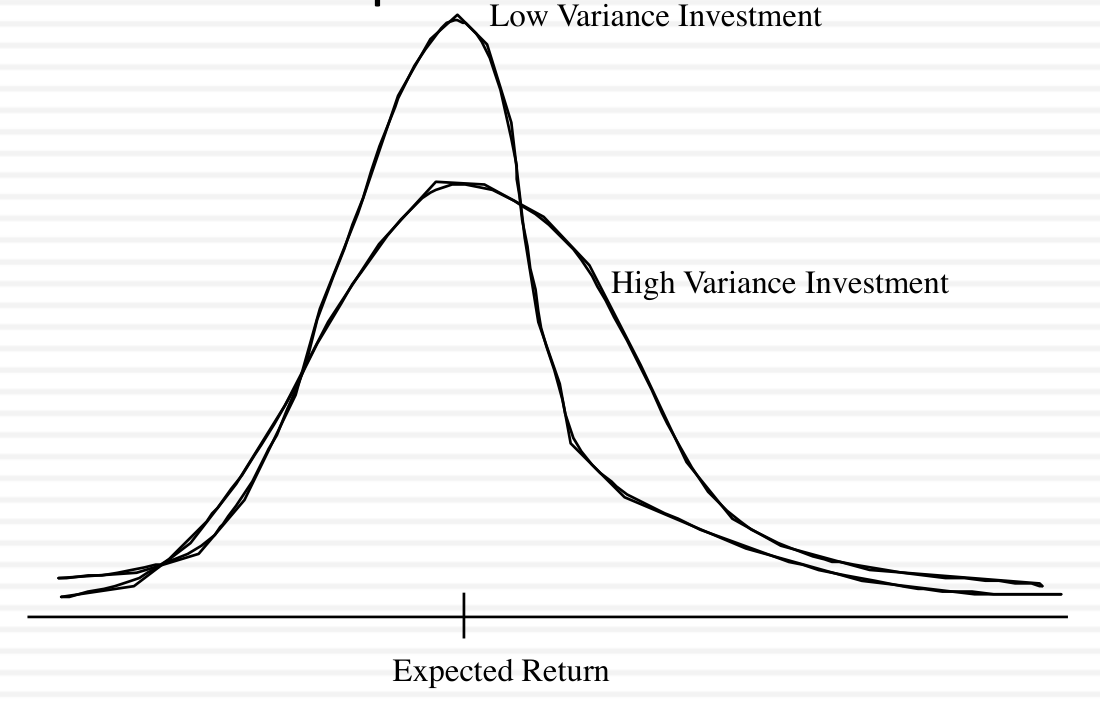
\includegraphics[width=\linewidth,height=0.6\textheight,keepaspectratio]{gfx/m2l1_damodaran_slide74_mean_variance.png}
\par\smallskip{\small 1. Khung Trung bình - Phương sai (Biểu đồ)}
\end{figure}

Khoản đầu tư có Phương sai Thấp (Low Variance Investment)

Khoản đầu tư có Phương sai Cao (High Variance Investment)

Lợi suất Kỳ vọng (Expected Return)

Aswath Damodaran 74

% [PDF p.76 | in p.75]
\section{Disney rủi ro đến mức nào? Một cái nhìn về quá khứ... (How risky is Disney? A look at the past\ldots{})}

\begin{figure}[H]
\centering
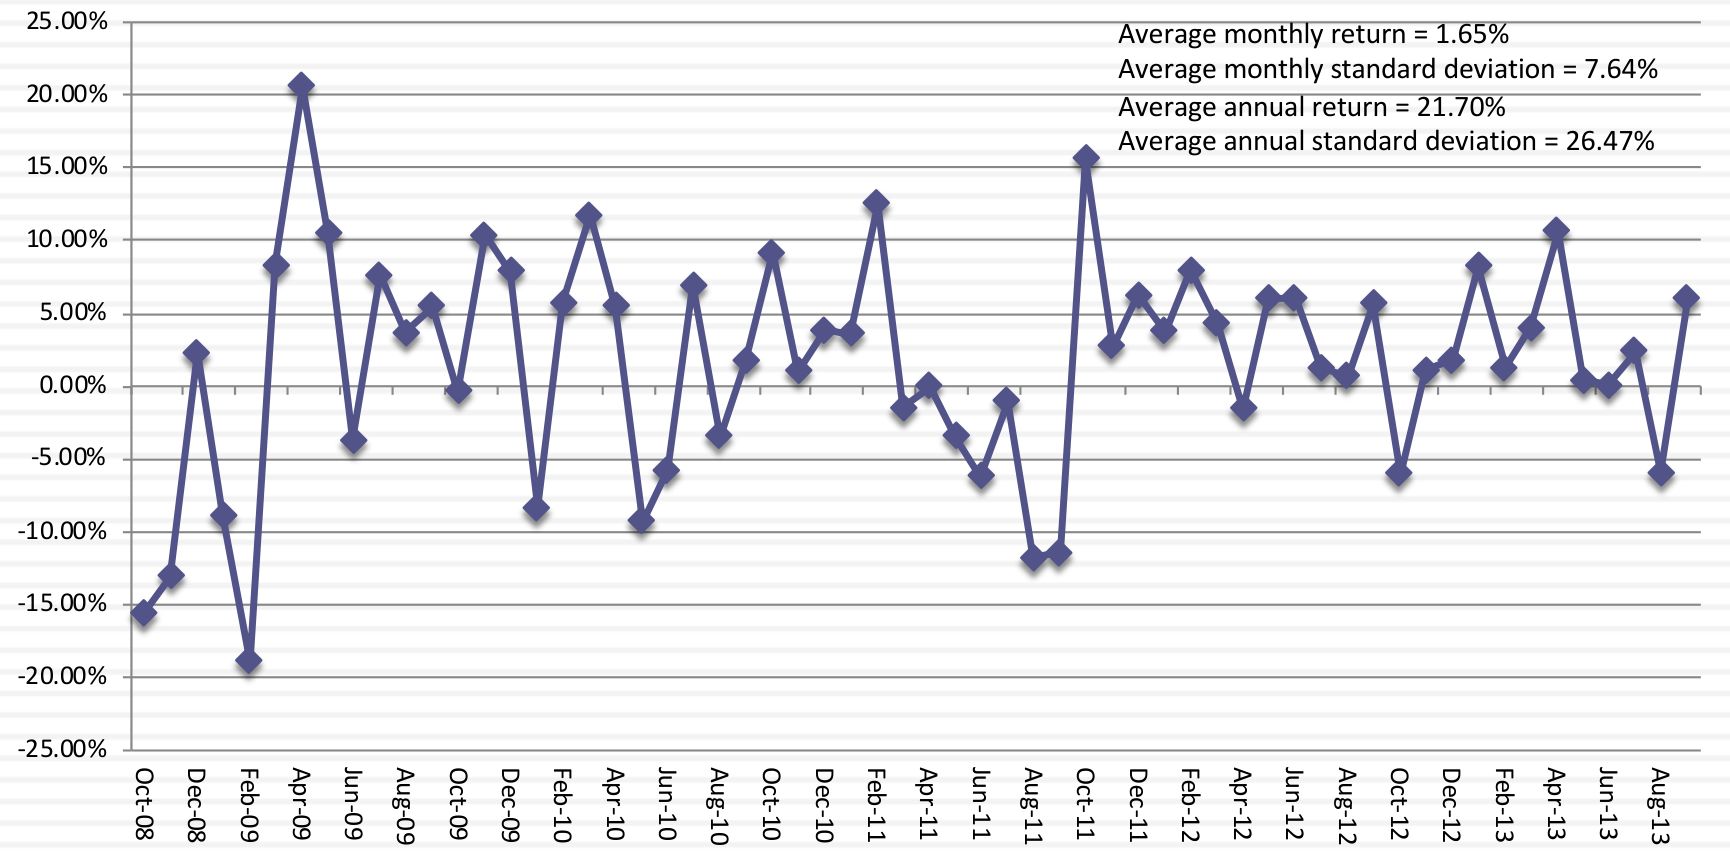
\includegraphics[width=\linewidth,height=0.6\textheight,keepaspectratio]{gfx/m2l1_damodaran_slide75_disney_risk.png}
\par\smallskip{\small Disney rủi ro đến mức nào? Một cái nhìn về quá khứ... (Biểu đồ)}
\end{figure}

Lợi suất của Disney - 2008-2013

Lợi suất trung bình hàng tháng = 1.65\% Độ lệch chuẩn (standard deviation) trung bình hàng tháng = 7.64\% Lợi suất trung bình hàng năm = 21.70\% Độ lệch chuẩn trung bình hàng năm = 26.47\%

Aswath Damodaran 75

% [PDF p.77 | in p.76]
\section{Bạn có sống trong thế giới trung bình - phương sai không? (Do you live in a mean-variance world?)}

\begin{itemize}
  \item Giả sử bạn phải chọn giữa hai khoản đầu tư. Chúng có cùng mức lợi suất kỳ vọng là 15\% và cùng độ lệch chuẩn là 25\%; tuy nhiên, khoản đầu tư A mang lại một khả năng rất nhỏ để bạn có thể nhân bốn (quadruple) số tiền của mình, trong khi mức chi trả (payoff) cao nhất có thể có của khoản đầu tư B là lợi suất 60\%. Bạn sẽ: a. bàng quan (indifferent) giữa hai khoản đầu tư, vì chúng có cùng mức lợi suất kỳ vọng và độ lệch chuẩn? b. ưa thích (prefer) khoản đầu tư A hơn, vì khả năng có mức chi trả cao? c. ưa thích (prefer) khoản đầu tư B hơn, vì nó an toàn hơn?
  \item Câu trả lời của bạn có thay đổi không nếu bạn không được cho biết rằng có một khả năng nhỏ là bạn có thể mất 100\% số tiền của mình vào khoản đầu tư A nhưng kịch bản tồi tệ nhất (worst case scenario) của bạn với khoản đầu tư B là -50\%?
\end{itemize}
Aswath Damodaran 76
